\documentclass[12pt,oneside,a4paper]{article}
\usepackage[usenames,dvipsnames]{color}
\usepackage[utf8]{inputenc}
\usepackage[T1]{fontenc}
\usepackage{lmodern}
\usepackage{graphicx}
\usepackage{wrapfig}
\usepackage{caption}
\usepackage{float}
\usepackage{subcaption}
\title{Notification\& Commentaire\\}
\author{Ben Rajeb Moncef,\\
        Université de Jean Monnet}

\begin{document}
% generates the title
\maketitle
% insert the table of contents
\tableofcontents
\maketitle
\newpage
\section{Introdutction}
\paragraph{}
Dans une autre phase d'implémentation de la plateforme, comme autres réseaux sociaux il est indisponsable de notifier l'utilisateur dans le cas du partage d'un stample, une catégorie, le demande d'ajout...
\paragraph{}
Stample offre la possibiliter d'organiser le contenu sous forme des catégories, le partage de de ces dérnier c'est une nouvelle fonctionnalité qu'on trouve sur dropbox, sauf que pour Stample les catégories sont organisées sous forme d'une arborescence similaire à un système de fichier.
\newline
Le stample ou autrement l'article c'est un contenu qui peut être écrit en précisant le titre, le contenu, l'auteur, la source....
Peut être aussi générer par des darg \& drop en utilisant le clipper depuis un autre site.
\paragraph{}
Ces options nécessitent d'informer les utilisateurs de la plateforme en option avec l'email et sous forme d'une alert sur le site.
\newline
La discution ou les commentaires sur un stample est aussi une fonctionnalité interessante pour interragir avec leur contenu.
Dans cette partie j'ai travaillé sur des sous tâches pour les Notifications, et des tests d'intégrations pour les commentaires.
\section{Notifications}
Le systéme de notification représente dans la base mongo par une collection notification\_inbox cette dernière elle se compose d'un ID, notification et isRead.
On utilise des servises : addNotificationsForUser, getNotificationForUser, deleteNotification, readNotification.
\section{Commentaires}
Pour partie des commentaires, j'ai eu l'implémentation des tests d'intégrations et des sous méthodes.
Les tests sont écritent en Specs2 (software specification for Scala) : c'est une librérie pour écrire des spécifications des softwares executables et lancer sur la console avec sbt "it:test".
Vous trouverez par suite deux captures d'écran une pour le lancement du test sbt et l'autre du code.
Il faut ajouter les dependencies du plugin dans le fichier ApplicationBuilt du projet.

\begin{figure}[H]
\begin{minipage}[c]{.7\linewidth}
\begin{center}
\fbox{
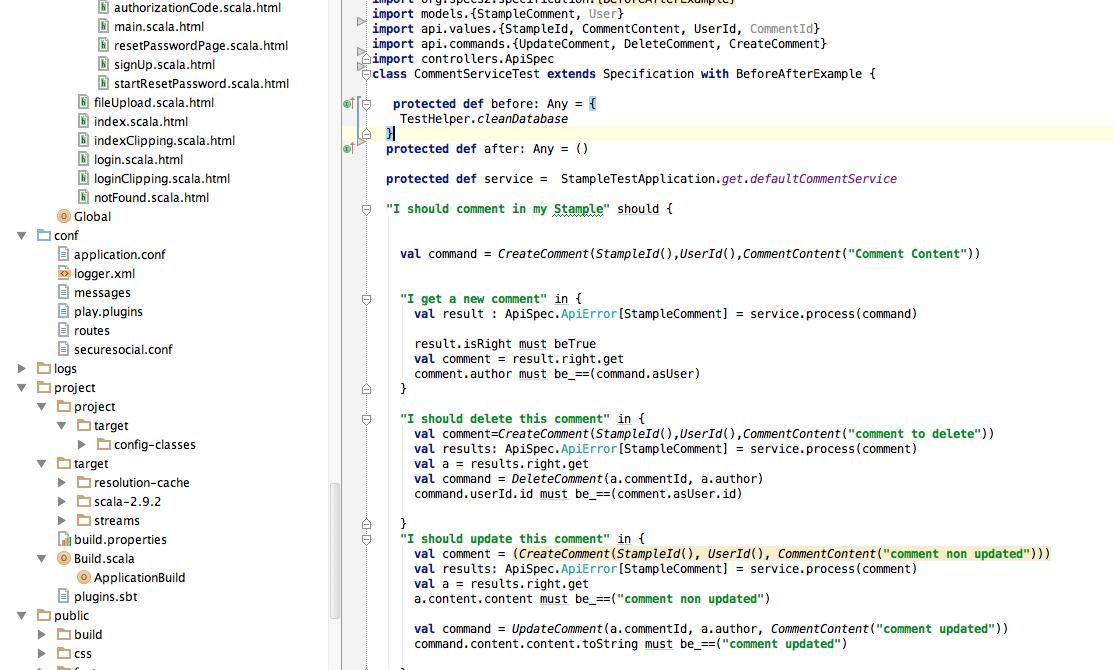
\includegraphics[width=14cm,height=100mm,scale=1]{test.png}}
\caption{Tests code}
\label{fig:Tests code}
\end{center}
\end{minipage}
\hfill
\begin{minipage}[c]{.5\linewidth}
\begin{center}
\fbox{
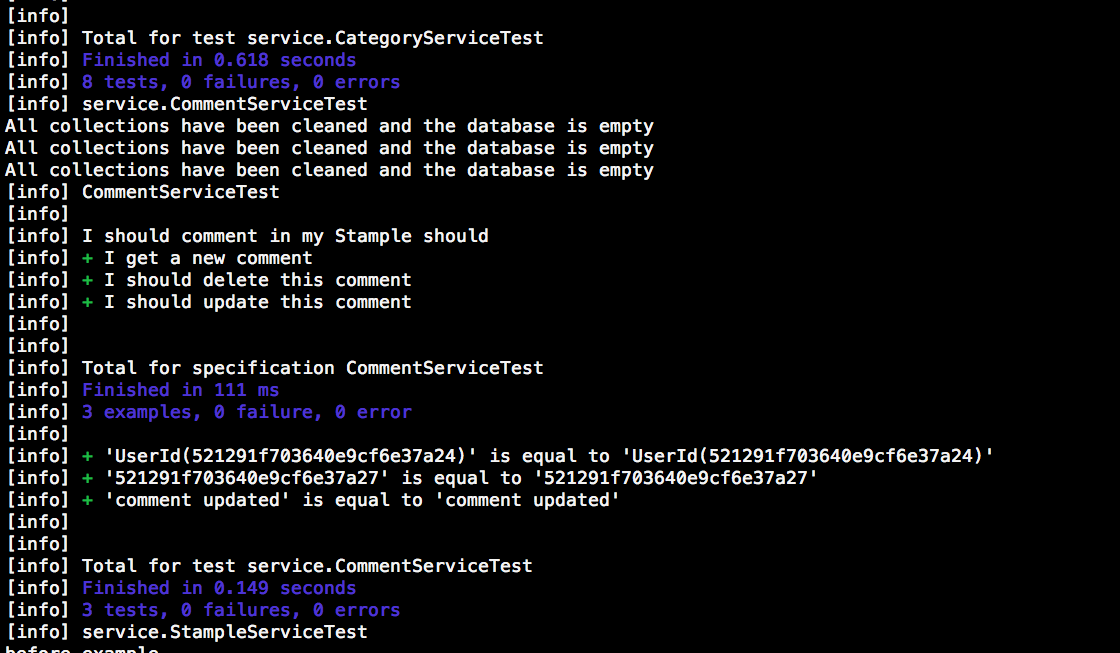
\includegraphics[width=14cm,height=100mm,scale=1]{code.png}}\hspace{1em}
\caption{Terminal lance tests}
\label{fig:Terminal lance tests}
\end{center}
\end{minipage}
\end{figure}

\section{Conclusion}
Dans cette partie du Stage, j'ai découvet le systéme de notification en travaillant sur des sous tâches, une première approche pour le commentStample et j'ai écris les tests nécessaires pour la creation, la mise à jour et la suppression des commentaires.
Le chapitre postérieur sera des altérnatives sur les reséaux sociaux centralisées et distribuées relative un future Stample en cours de construction.
Des bibliothéques sont misent en ligne un projet open source "banana-rdf" et "RWW-Play", Henry Story, travaille sur ces bibliothéques pour les adaptées au plateforme Stample.


  
\end{document}